\section{Sarkaç}

\begin{justify}
Okulda incelediğiniz ilk doğrusal olmayan sistem muhtemelen sarkaçtı. Ancak temel derslerde sarkacın asıl doğrusal olmayan yapısı genellikle küçük açı yaklaşımı $\sin\theta\approx\theta$ ile geçiştirilir. Bu bölümde faz düzlemi yöntemleri kullanılarak sarkaç, büyük açı rejimi de dâhil olmak üzere incelenir.

Sönüm ve dış zorlama yokken sarkacın hareketi
\begin{equation}
\frac{d^2\theta}{dt^2}+\frac{g}{L}\sin\theta=0
\end{equation}
ile verilir. Burada $\theta$ aşağı düşey doğrultudan ölçülen açı, $g$ yerçekimi ivmesi ve $L$ sarkacın uzunluğudur (Şekil~\ref{fig:6-7-1}).

\begin{figure}[H]
\centering
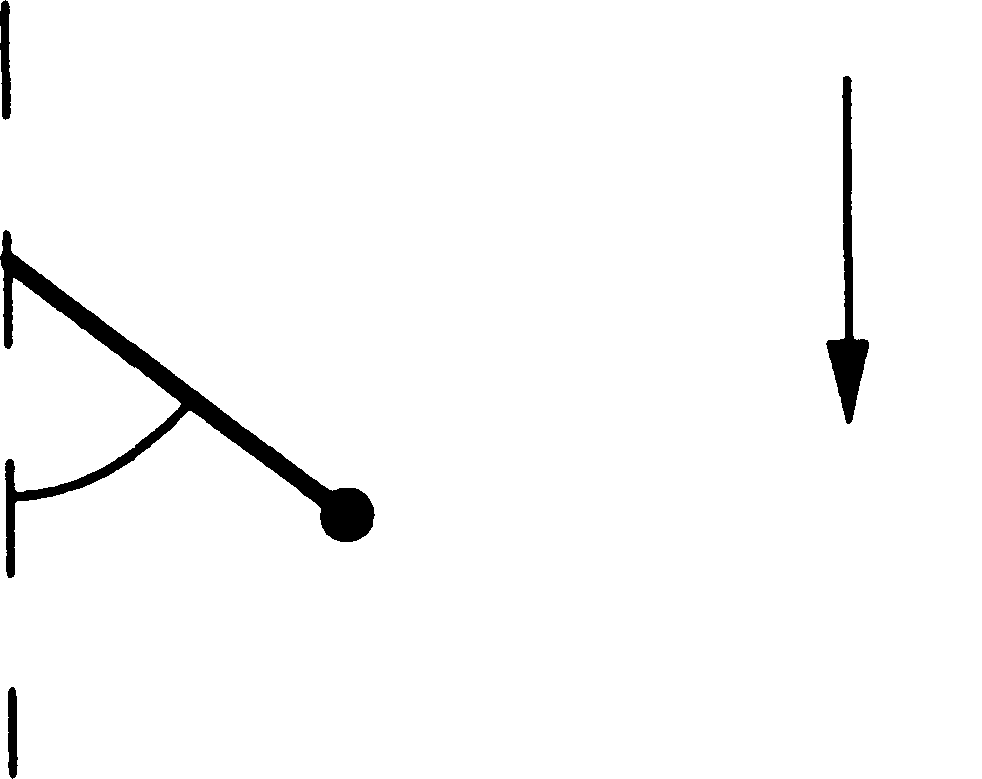
\includegraphics[width=0.82\textwidth]{images/Figures/figur-027.png}
\caption{Sarkacın geometrisi ve açı tanımı.}
\label{fig:6-7-1}
\end{figure}

Boyutsuzlaştırma için $\omega=\sqrt{g/L}$ ve $\tau=\omega t$ tanımlanır. Böylece denklem
\begin{equation}
\ddot{\theta}+\sin\theta=0
\end{equation}
hâline gelir; burada nokta $\tau$'ya göre türevi gösterir. Faz düzlemindeki karşılık gelen sistem
\begin{align}
\dot{\theta} &= v,\\
\dot{v} &= -\sin\theta
\end{align}
şeklindedir. Burada $v$ boyutsuz açısal hızdır.

Sabit noktalar $(\theta^{*},v^{*})=(k\pi,0)$ noktalarıdır; burada $k$ herhangi bir tam sayıdır. $2\pi$ kadar farklı olan açılar fiziksel olarak aynı olduğundan, $(0,0)$ ve $(\pi,0)$ noktalarına odaklanmak yeterlidir.

$(0,0)$ noktasında Jacobian
\begin{equation}
A=\begin{pmatrix}0&1\\-1&0\end{pmatrix}
\end{equation}
olur. Bu nedenle orijin doğrusal bir merkezdir. Aslında orijin doğrusal olmayan bir merkezdir. Bunun iki nedeni vardır: Sistem tersinirdir; $\tau\mapsto -\tau$, $v\mapsto -v$ dönüşümü altında denklemler değişmez. Ayrıca sistem korunumludur. Denklem $\dot{\theta}$ ile çarpılıp integre edilirse
\begin{equation}
\frac{1}{2}\dot{\theta}^{2}-\cos\theta=\text{sabit}
\end{equation}
bulunur. Enerji fonksiyonu
\begin{equation}
E(\theta,v)=\frac{1}{2}v^2-\cos\theta
\end{equation}
şeklindedir. Bu fonksiyonun $(0,0)$ noktasında yerel minimumu vardır; dolayısıyla orijin doğrusal olmayan bir merkezdir.

Şimdi sarkacı ters konumda, yani $(\pi,0)$ noktasında düşünelim. Bu noktadaki Jacobian
\begin{equation}
A=\begin{pmatrix}0&1\\1&0\end{pmatrix}
\end{equation}
olur. Karakteristik denklem $\lambda^2-1=0$ olduğundan $\lambda_1=-1$, $\lambda_2=1$ bulunur. Bu nokta bir eyer noktasıdır. Karşılık gelen özvektörler $(-1,1)$ ve $(1,1)$ doğrultularıdır.

Sabit noktalar yakınındaki faz portresi Şekil~\ref{fig:6-7-2}'de, enerji konturlarının eklenmesiyle elde edilen faz portresi ise Şekil~\ref{fig:6-7-3}'te gösterilecektir.

\begin{figure}[H]
\centering
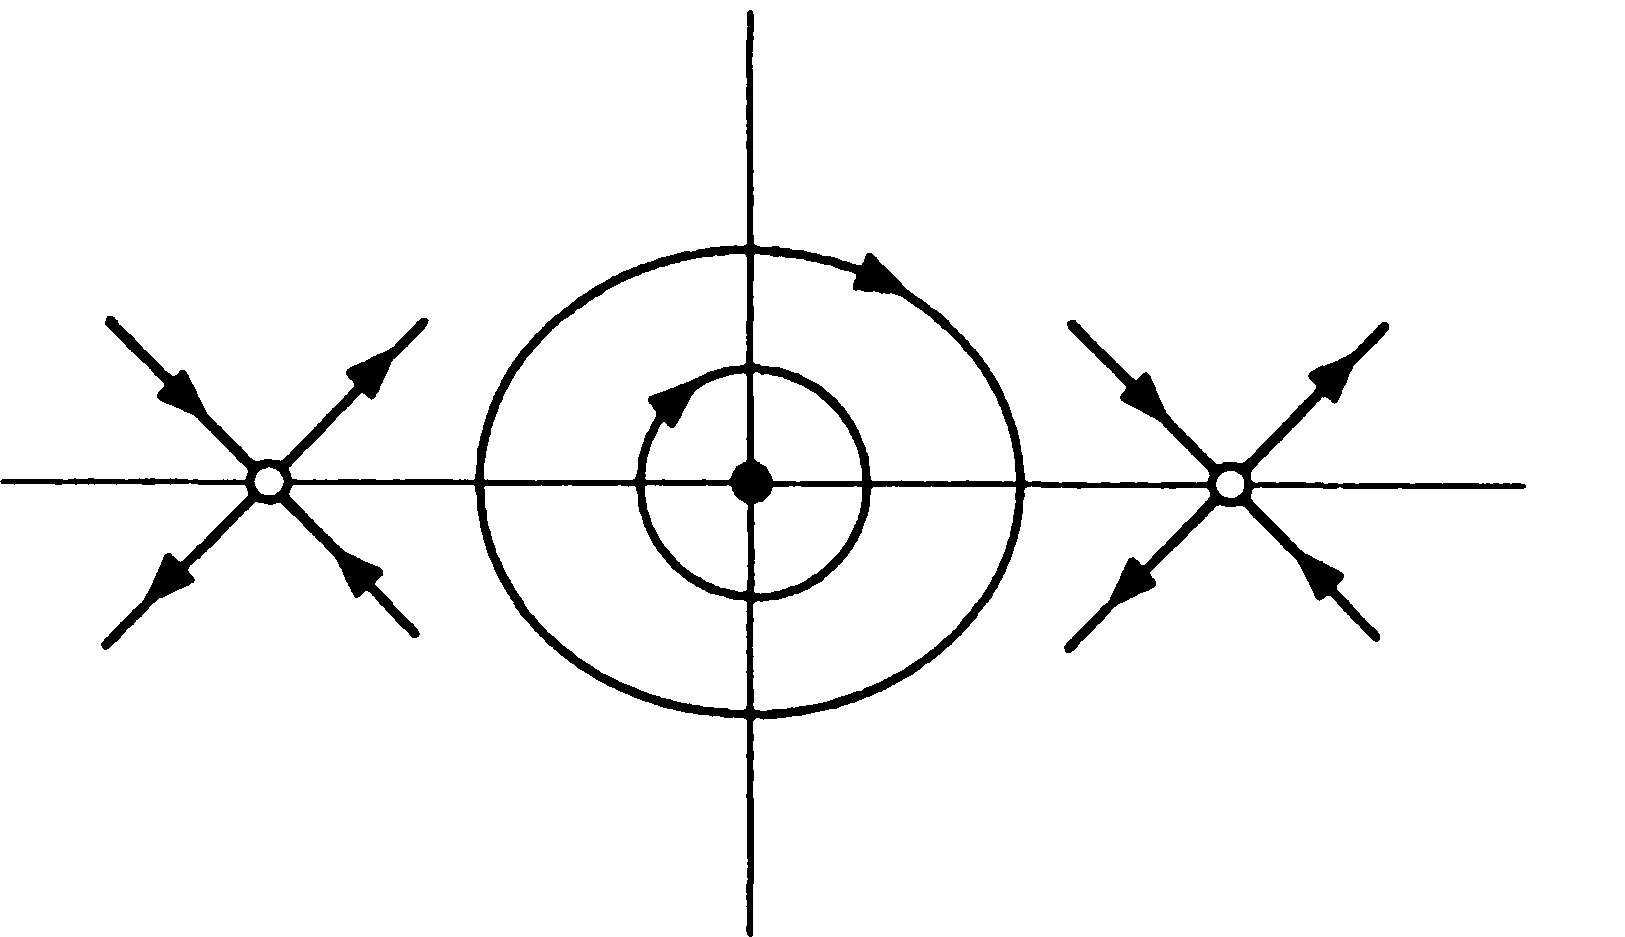
\includegraphics[width=0.82\textwidth]{images/Figures/figur-028.png}
\caption{Sarkaçta merkez ve eyer noktaları yakınındaki yerel faz portresi.}
\label{fig:6-7-2}
\end{figure}
\begin{figure}[H]
\centering
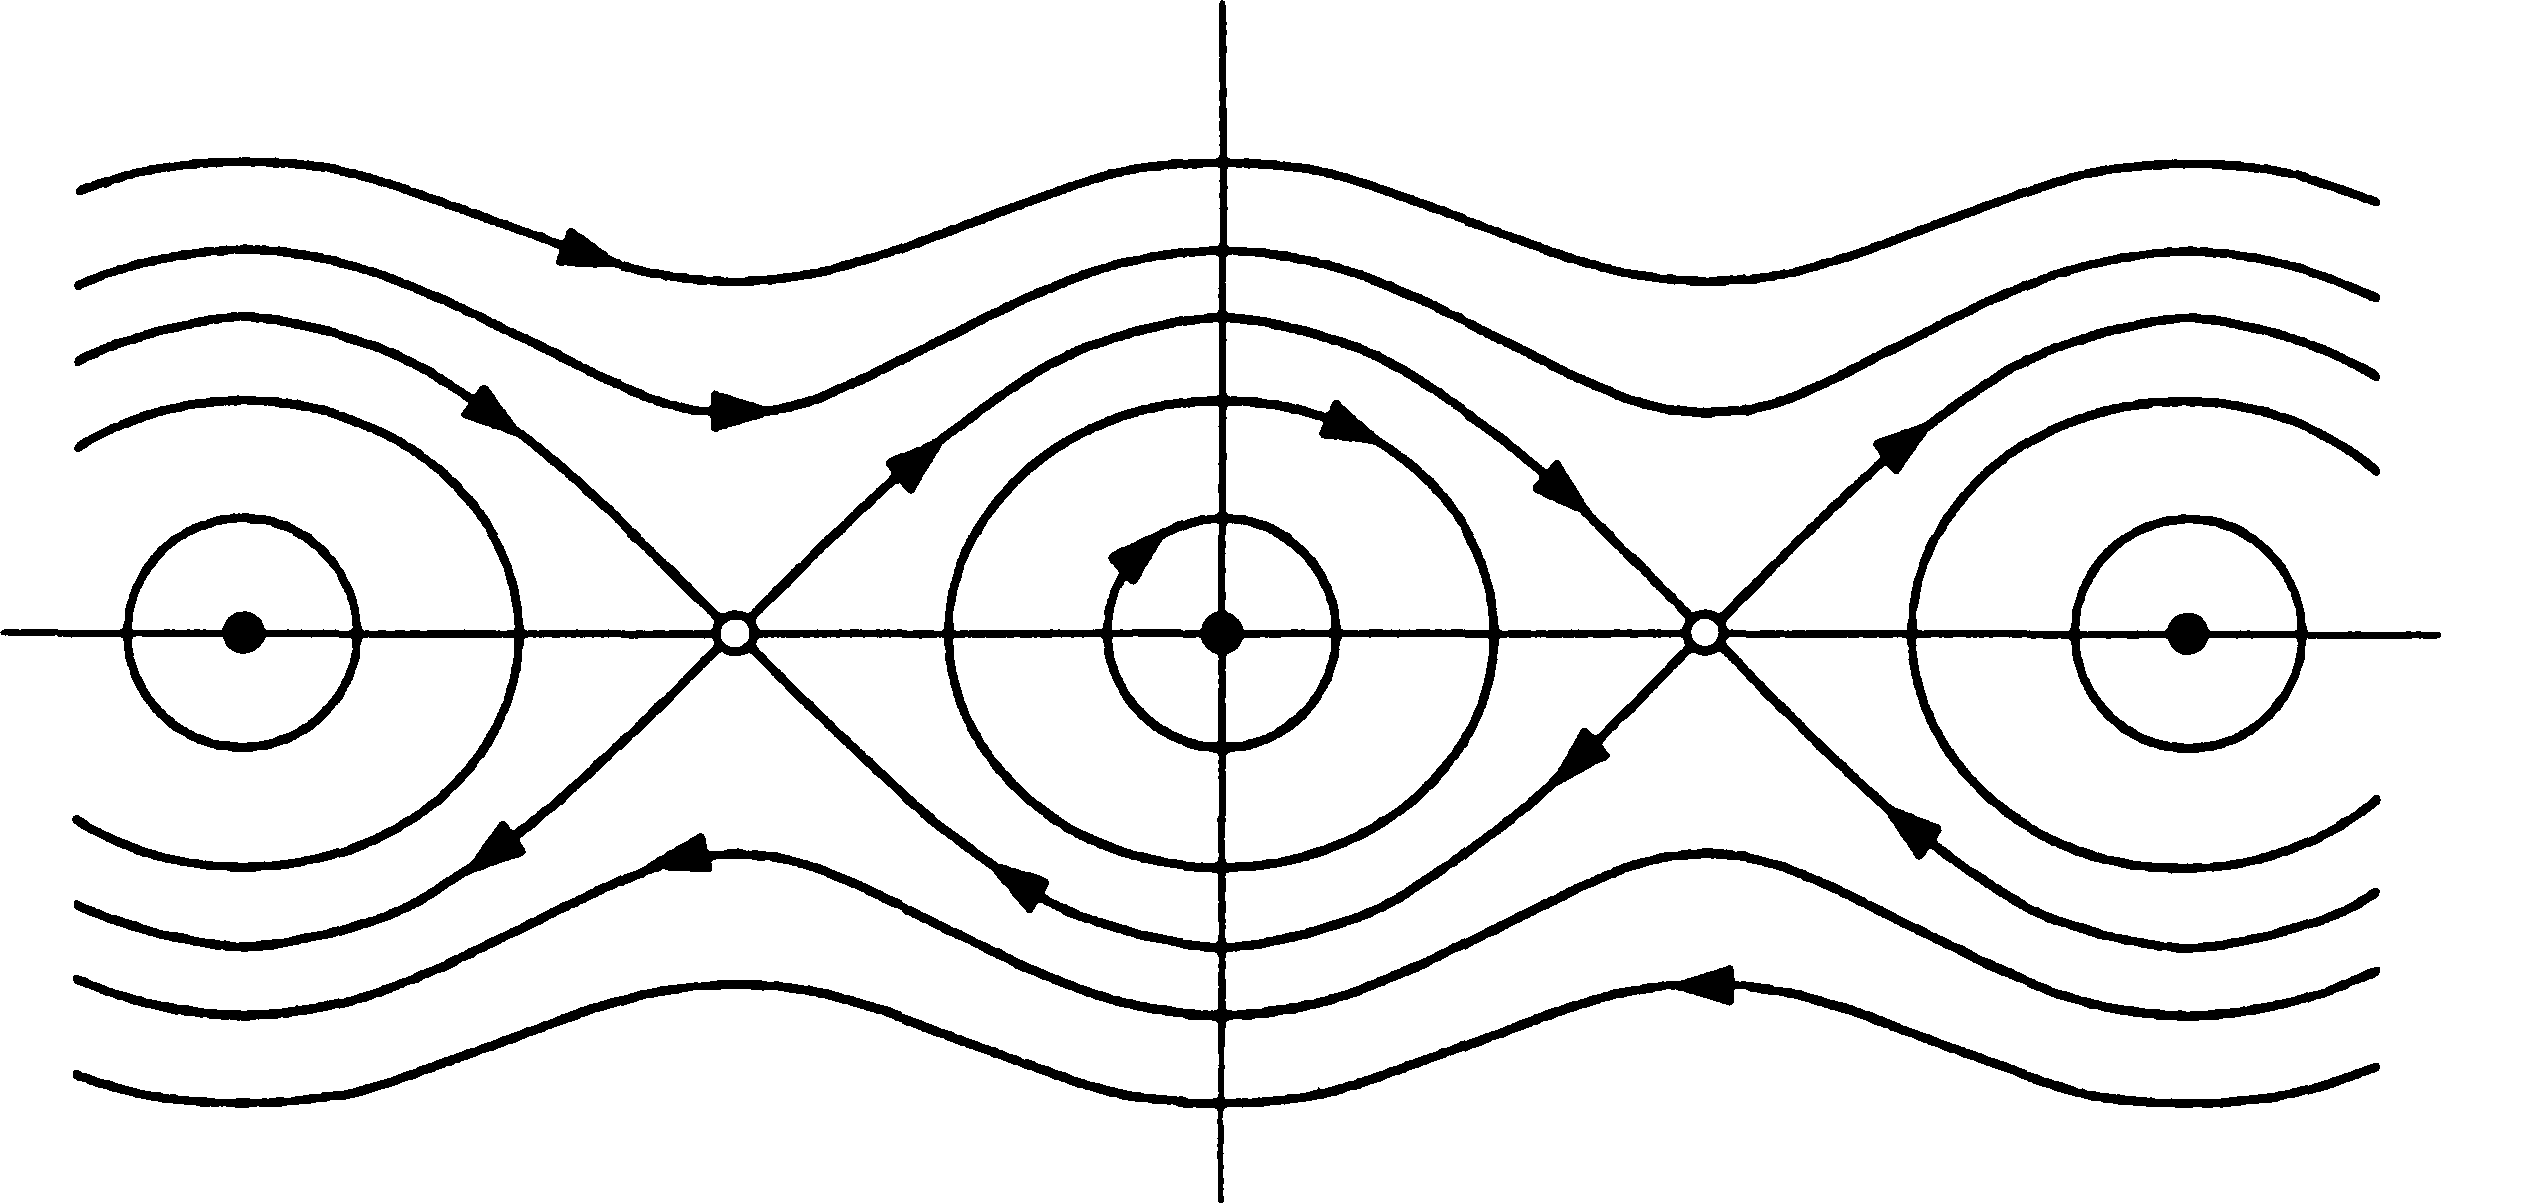
\includegraphics[width=0.82\textwidth]{images/Figures/figur-029.png}
\caption{Sönümsüz sarkaç için enerji konturları ve faz portresi.}
\label{fig:6-7-3}
\end{figure}

Fiziksel yorum şöyledir: Merkez, sarkacın aşağı doğru asılı ve dengede olduğu nötr kararlı duruma karşılık gelir. Bu en düşük enerji durumudur. Merkez çevresindeki küçük kapalı yörüngeler küçük salınımları temsil eder. $E=1$ kritik durumu, eyerleri birleştiren heteroklinik yörüngelere karşılık gelir. Bu yörüngeler ters çevrilmiş sarkaç durumunda hassas hareketleri temsil eder. $E>1$ olduğunda sarkaç tepeyi tekrar tekrar aşarak döner.
\end{justify}

\subsection*{Silindirik Faz Uzayı}
\addcontentsline{toc}{subsection}{Silindirik Faz Uzayı}

\begin{justify}
Sarkacın faz portresi, silindir yüzeyine sarıldığında daha aydınlatıcı olur (Şekil~\ref{fig:6-7-4}). Gerçekte sarkaç için doğal faz uzayı silindirdir; çünkü açısal hız $v$ gerçek bir sayı iken $\theta$ bir açıdır.

\begin{figure}[H]
\centering
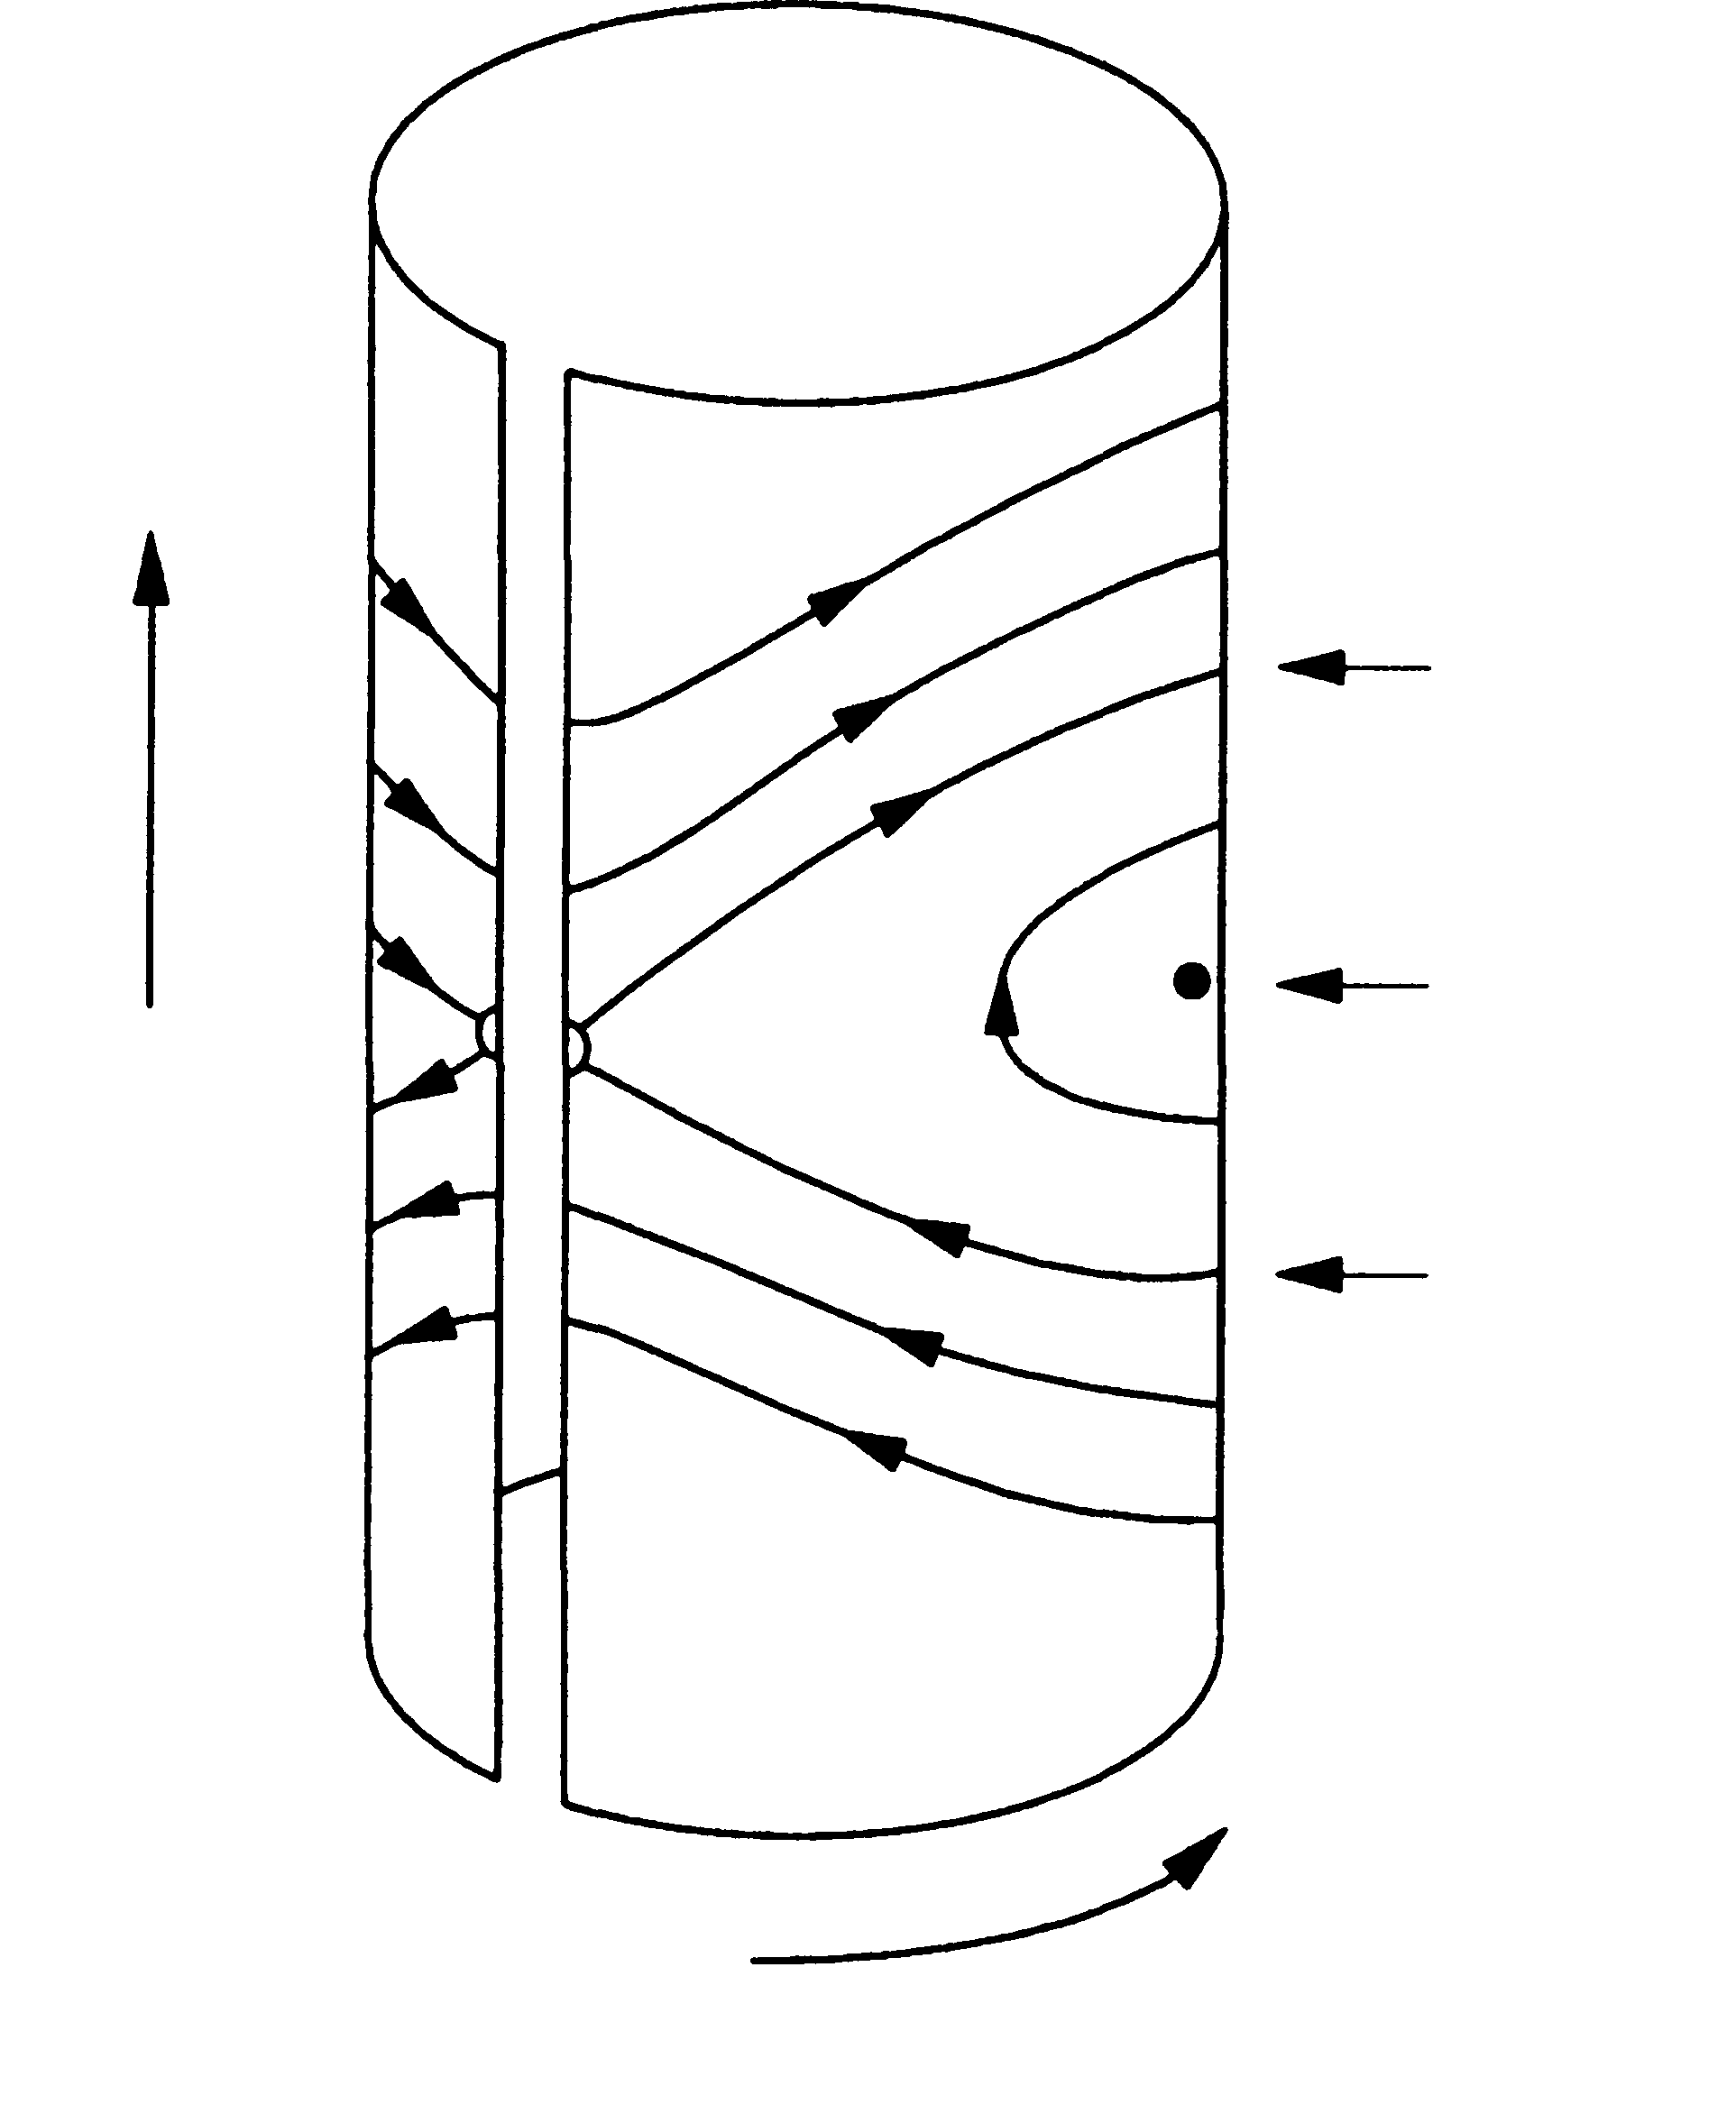
\includegraphics[width=0.82\textwidth]{images/Figures/figur-030.png}
\caption{Sarkacın silindirik faz uzayındaki faz portresi.}
\label{fig:6-7-4}
\end{figure}

Silindirik gösterimin birkaç avantajı vardır. $E>1$ için periyodik dönme hareketleri artık gerçekten periyodik görünür; bunlar silindiri çevreleyen kapalı yörüngelerdir. Ayrıca Şekil~\ref{fig:6-7-3}'teki eyer noktalarının fiziksel olarak aynı durumu, yani tepe konumunda duran ters sarkacı temsil ettiği açık hâle gelir. Düzlemde heteroklinik görünen yörüngeler silindir üzerinde homoklinik yörüngelere dönüşür.

Enerjiyi açısal hız yerine dikey eksende çizmek simetriyi daha açık gösterir. Bu durumda yörüngeler sabit yükseklikte kalırken silindir U biçimli bir tüpe bükülür (Şekil~\ref{fig:6-7-5}). Tüpün iki kolu sarkacın saat yönünde ya da saat yönünün tersinde dönmesini temsil eder. Düşük enerjilerde bu ayrım ortadan kalkar; sarkaç ileri geri salınır. Homoklinik yörüngeler $E=1$ seviyesinde, dönmeler ile salınımlar arasındaki sınırda bulunur.

\begin{figure}[H]
\centering
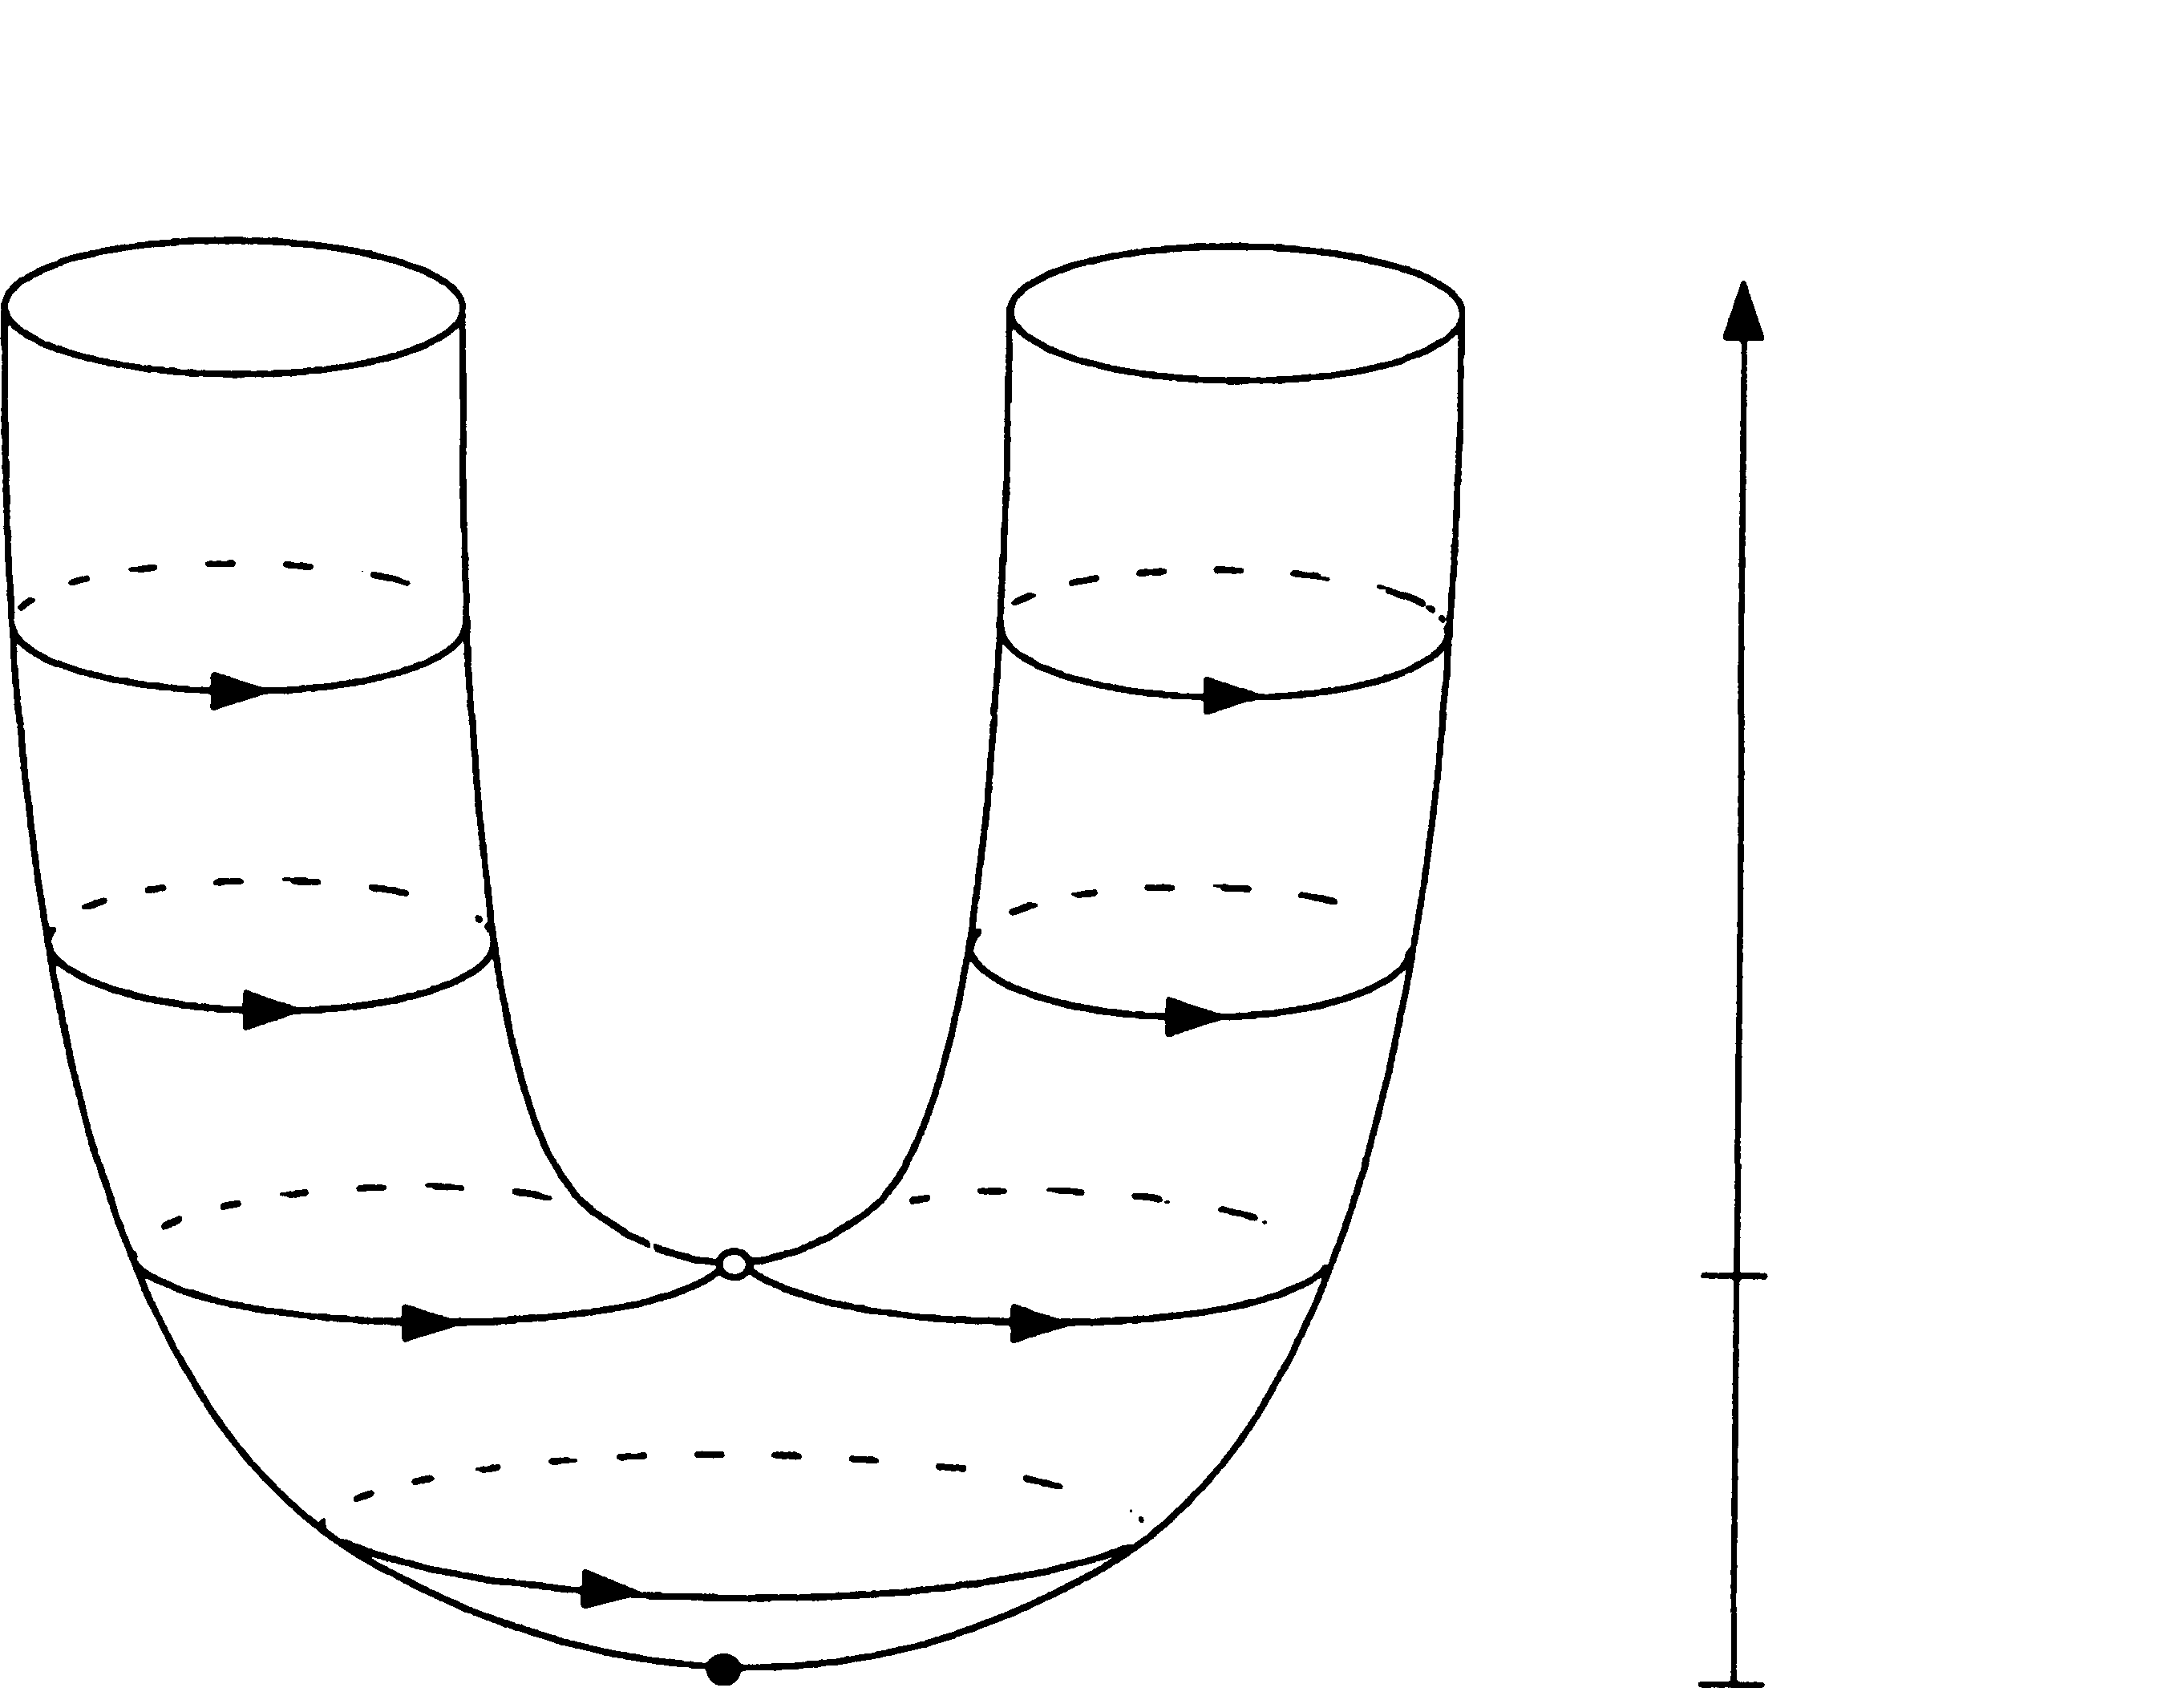
\includegraphics[width=0.82\textwidth]{images/Figures/figur-031.png}
\caption{Enerjinin dikey eksende çizildiği U-tüp gösterimi.}
\label{fig:6-7-5}
\end{figure}

İlk bakışta U-tüpün kollarından birindeki oklar ters çizilmiş gibi görünebilir. Ancak koordinat sistemine bakıldığında çizimin doğru olduğu anlaşılır (Şekil~\ref{fig:6-7-6}). Silindirin alt kısmı U-tüp oluşturacak biçimde büküldüğünde artan $\theta$ yönü tersine dönmüştür.

\begin{figure}[H]
\centering
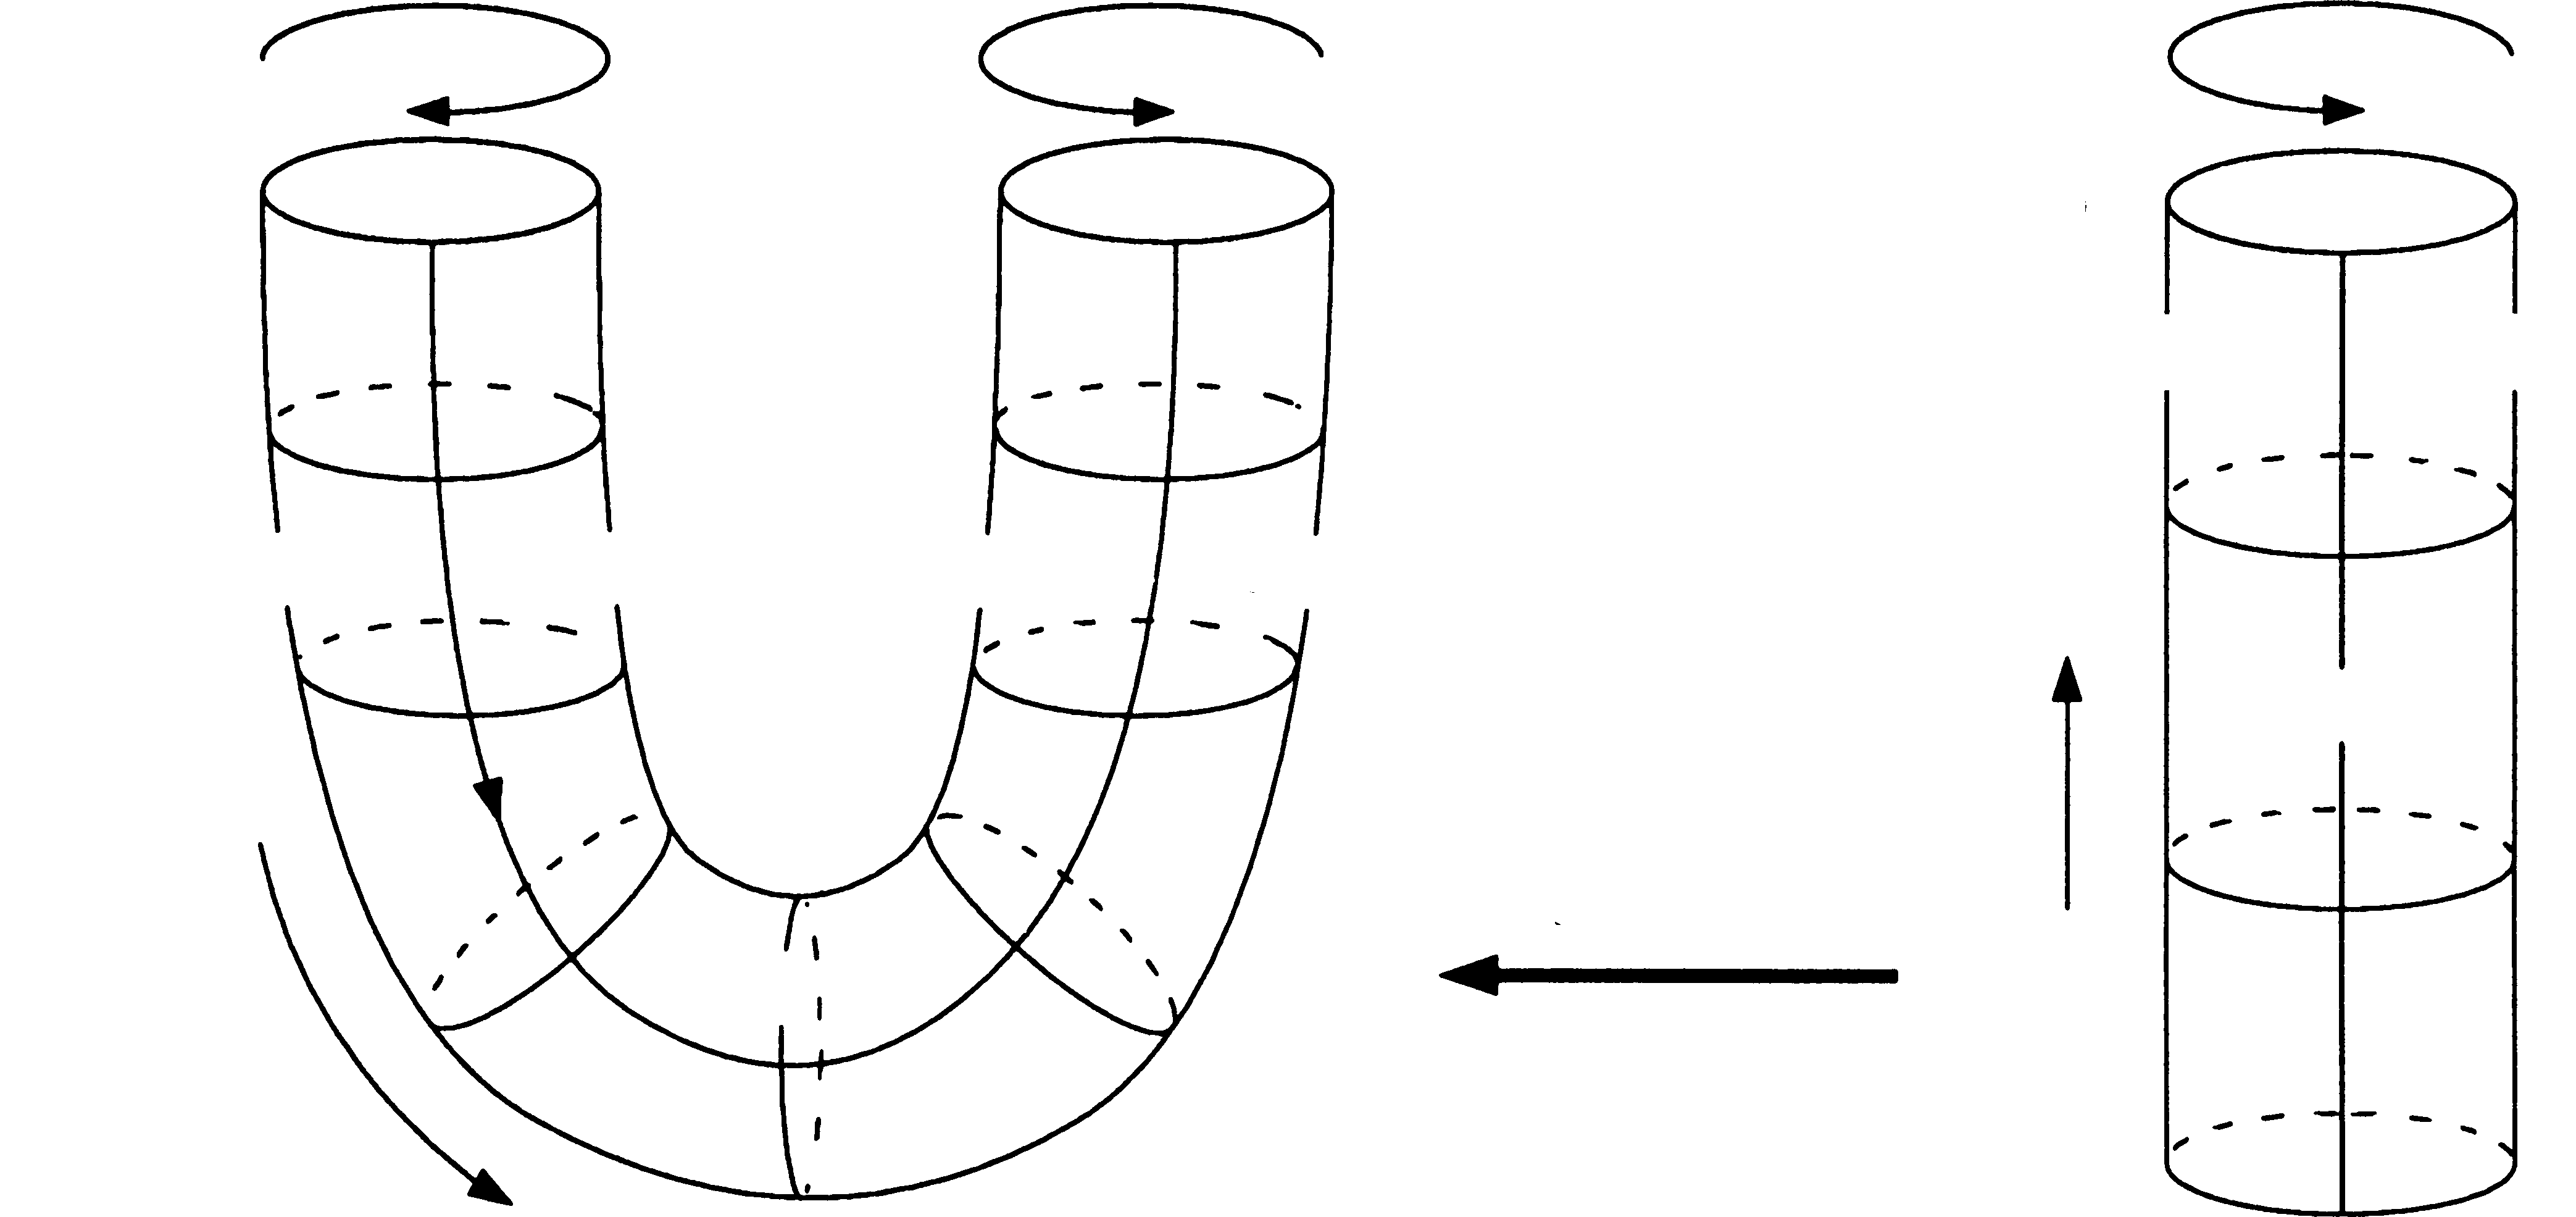
\includegraphics[width=0.82\textwidth]{images/Figures/figur-032.png}
\caption{Silindirik koordinat sisteminin U-tüp gösterimine bükülmesi.}
\label{fig:6-7-6}
\end{figure}
\end{justify}

\subsection*{Sönüm}
\addcontentsline{toc}{subsection}{Sönüm}

\begin{justify}
Şimdi faz düzlemine geri dönelim ve sarkaca küçük miktarda doğrusal sönüm ekleyelim. Denklem
\begin{equation}
\ddot{\theta}+b\dot{\theta}+\sin\theta=0
\end{equation}
olur; burada $b>0$ sönüm şiddetidir. Bu durumda merkezler kararlı spirallere dönüşürken eyerler eyer olarak kalır. Bilgisayar üretimli faz portresi Şekil~\ref{fig:6-7-7}'de gösterilecektir.

\begin{figure}[H]
\centering
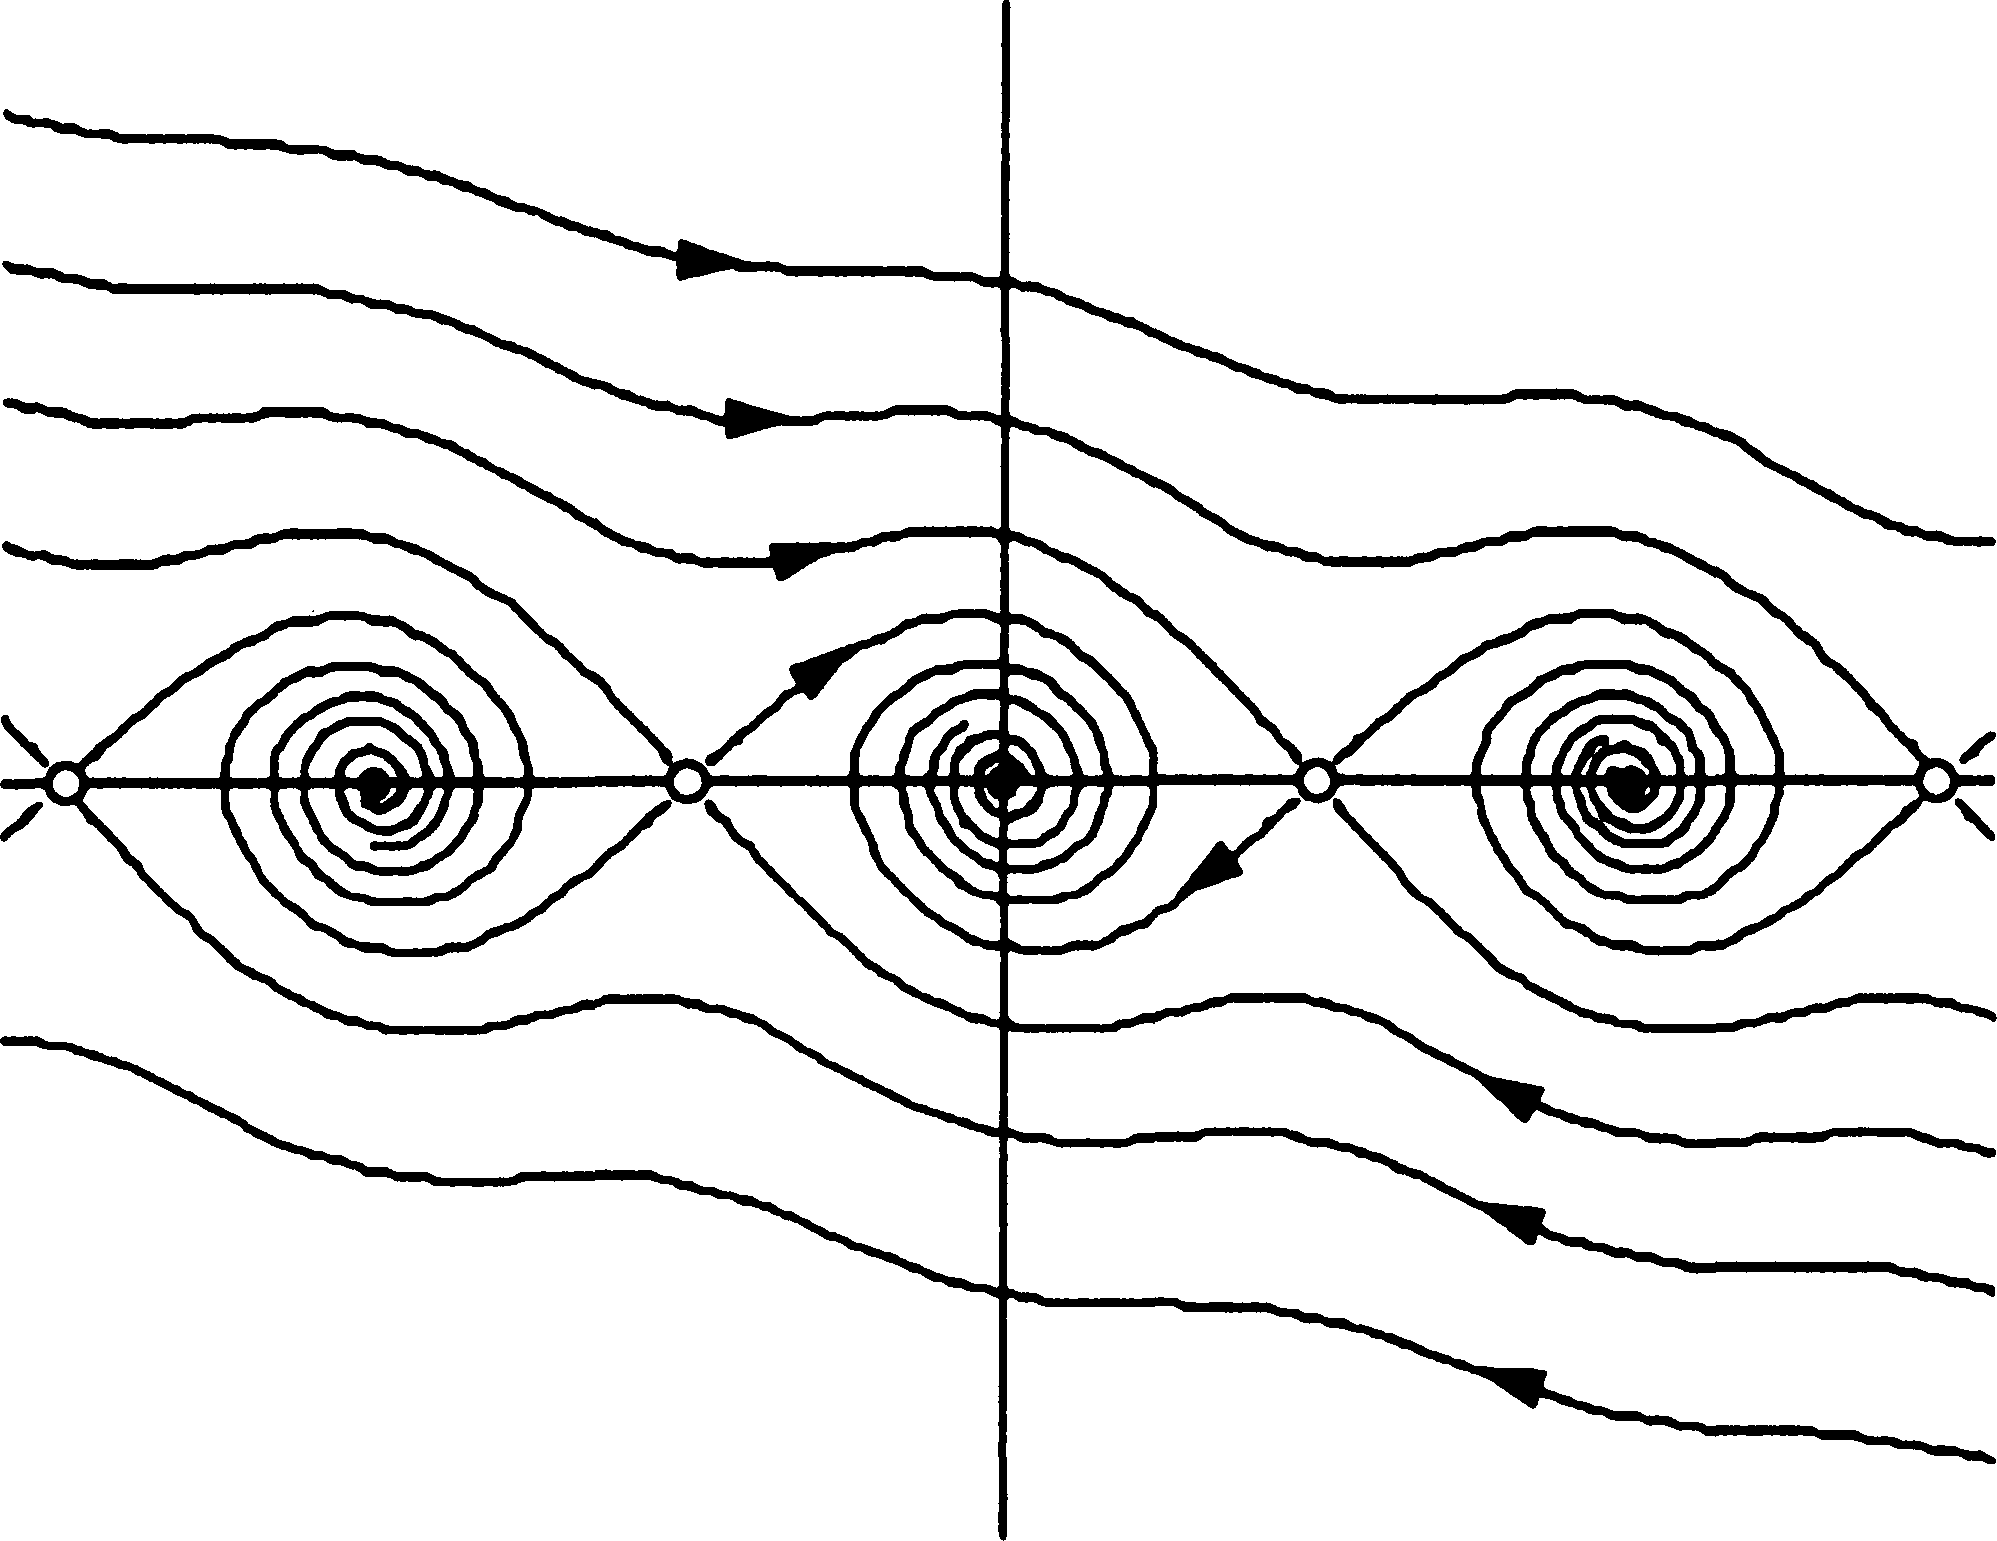
\includegraphics[width=0.82\textwidth]{images/Figures/figur-033.png}
\caption{Sönümlü sarkaç için faz portresi.}
\label{fig:6-7-7}
\end{figure}

U-tüp gösteriminde durum daha açıktır: sabit noktalar dışında tüm yörüngeler sürekli irtifa kaybeder (Şekil~\ref{fig:6-7-8}). Enerjinin yörünge boyunca değişimi
\begin{equation}
\frac{dE}{d\tau}
=\frac{d}{d\tau}\left(\frac{1}{2}\dot{\theta}^2-\cos\theta\right)
=\dot{\theta}(\ddot{\theta}+\sin\theta)
=-b\dot{\theta}^{2}\le 0
\end{equation}
şeklindedir. Dolayısıyla sabit noktalar dışında enerji yörüngeler boyunca monoton olarak azalır.

\begin{figure}[H]
\centering
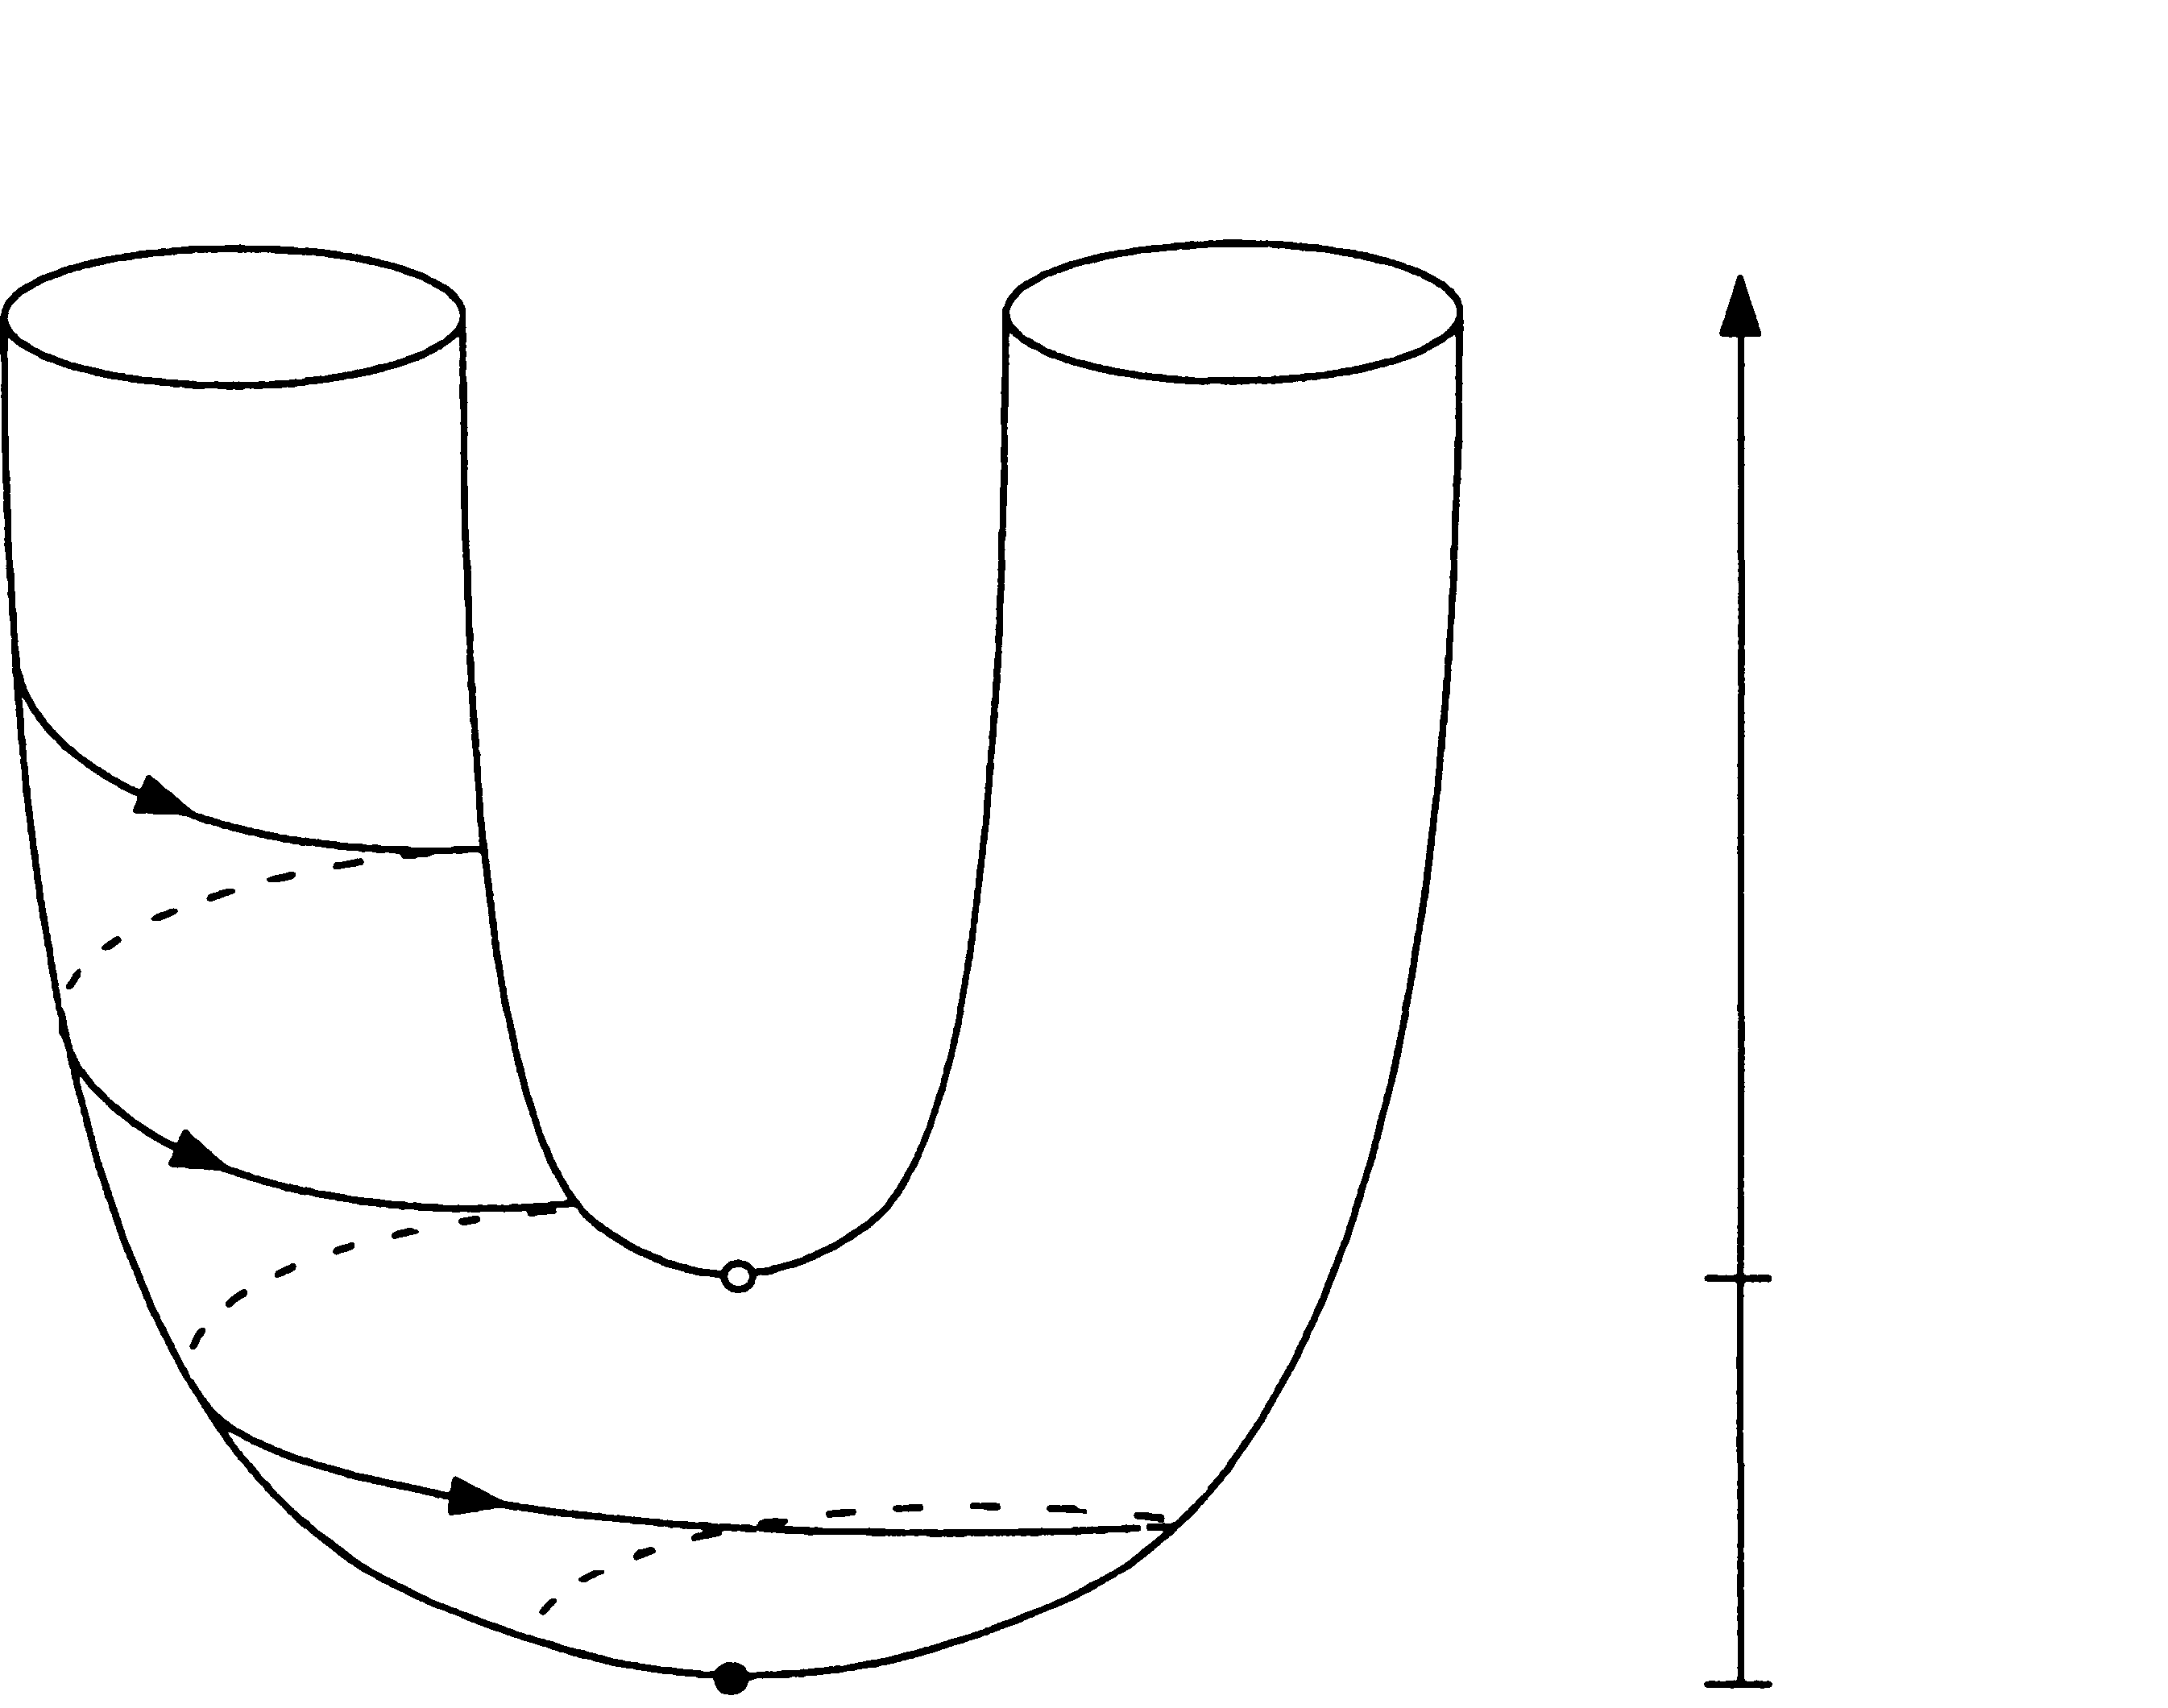
\includegraphics[width=0.82\textwidth]{images/Figures/figur-034.png}
\caption{Sönümlü sarkacın U-tüp enerji gösterimi.}
\label{fig:6-7-8}
\end{figure}

Şekil~\ref{fig:6-7-8}'deki yörüngenin fiziksel yorumu şudur: sarkaç başlangıçta saat yönünde dönmektedir. Enerji kaybettikçe tepeyi aşması zorlaşır. Karşılık gelen yörünge U-tüpün kolundan aşağı doğru spirallenir; $E<1$ olduğunda sarkaç artık dönemeyecek kadar az enerjiye sahiptir ve taban etrafında küçük salınımlara yerleşir. Sonunda hareket sönümlenir ve sarkaç kararlı dengesinde durur.

Bu örnek, yalnızca faz portresi resimleriyle sarkacın dinamiğinin temel özelliklerinin çıkarılabileceğini gösterir. Aynı sonuçları analitik formüllerle elde etmek çok daha zor ve yorumlamak daha karmaşık olurdu.
\end{justify}

\newpage